\documentclass[beamer]{standalone}

\usetheme{naked}
\setbeamercolor{alerted text}{fg=green!50!black}
\setbeamercolor{box title}{fg=purple}
\setbeamertemplate{frametitle}{}

% \usepackage{xkeyval}
% \usepackage{pgffor}

\usepackage{standalone}

\makeatletter
../code-graphs.tex
\makeatother

% vertical centering of cells
% see http://tex.stackexchange.com/questions/46386/vertically-center-cells-of-a-table
\usepackage{array}% http://ctan.org/pkg/array
\newcolumntype{M}{>{\centering\arraybackslash}m{\dimexpr.17\linewidth-2\tabcolsep}}

% remove space between margin and lists
\usepackage{enumitem}
\setitemize{label=\usebeamerfont*{itemize item}%
  \usebeamercolor[fg]{itemize item}
  \usebeamertemplate{itemize item}}
\setlist{leftmargin=*,labelindent=0cm}

%\usepackage{amsmath}

\usepackage{tikz}
\usepackage{tkz-graph}
\usepackage{tkz-berge}
\usepackage{tkz-berge-add}

\usepackage[utf8]{inputenc}
% \usepackage{libertine}
% \usepackage[libertine]{newtxmath}

%\usepackage{lxfonts}

\usepackage{cabin}
\usepackage{mathastext}

\newcommand{\graphcaption}[4][gray!80!white]{\draw (#2,#3) node [fill=#1]{#4};}

\SetVertexSimple[FillColor=gray, MinSize=10pt, LineWidth=1.5pt]

\tikzset{EdgeStyle/.style= {%
    color           = white,
    double          = black,
    double distance = 2.5pt}}

\newcommand{\setof}[2]{\left\{\,#1\mid #2\,\right\}}

\newcommand{\triangulo}[4]{%
  \shadedraw[inner color=#4,opacity=0.8,line width=1pt]
  (#1.center) -- (#2.center) -- (#3.center) -- cycle;}

\newcommand{\triangleshaded}[3]{%
  \draw[fill=gray]
  (#1.center) -- (#2.center) -- (#3.center) -- cycle;}

\newcommand{\triang}[3]{%
  \shadedraw[inner color=gray,,opacity=0.8,line width=1pt]
  (#1.center) -- (#2.center) -- (#3.center) -- cycle;}

\begin{document}
\begin{standaloneframe}
   \begin{center}
    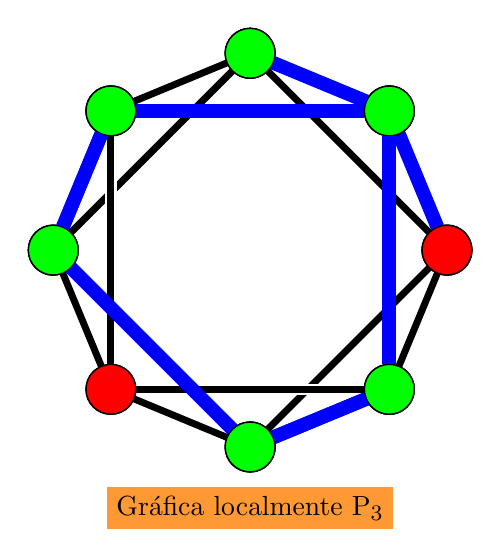
\begin{tikzpicture}
      \grCirculant[RA=2.5]{8}{1,2}
      \uncover<1-3>{\AddVertexColor{red}{a2}}
      \uncover<2,3>{\AddVertexColor{green}{a0,a1,a3,a4}}
      \uncover<3>{%
        \SetUpEdge[lw=5pt,color=blue]
        \Edge(a0)(a1)
        \Edge(a1)(a3)
        \Edge(a3)(a4)
        }
      \uncover<4>{
        \AddVertexColor{red}{a5}
        \AddVertexColor{green}{a3,a4,a6,a7}
        {\SetUpEdge[lw=5pt,color=blue]
          \Edge(a3)(a4)
          \Edge(a6)(a4)
          \Edge(a6)(a7)
        }
      }
      \uncover<5>{
        \AddVertexColor{red}{a0}
        \AddVertexColor{green}{a1,a2,a6,a7}
        {\SetUpEdge[lw=5pt,color=blue]
          \Edge(a1)(a2)
          \Edge(a7)(a1)
          \Edge(a6)(a7)
        }
      }
      \uncover<6>{\draw (0,-3) node [fill=orange!80!white,below]{Gráfica
        localmente $P_{3}$};}
    \end{tikzpicture}
  \end{center} 
\end{standaloneframe}
\end{document}
